\section{Electron--phonon matrix elements}\label{sec:6.2}

An electron at the bottom of the conduction band of GaAs absorbs a longitudinal optical phonon of wavevector \SI{0.01}{\angstrom^{-1}} with a vertex $|g| = \SI{3.3}{eV}$. An electron in a conduction valley of silicon absorbs a longitudinal sound wave of the same wavevector, running along the valley axis, with $|g| = \SI{26}{meV}$, more than a hundred times less. Ten times longer wavelengths make the GaAs vertex ten times larger and the silicon one $\sqrt{10}$ times smaller. Both numbers follow from the definition \cref{eq:6.1-Hep} once the bare potential of a displaced nucleus is replaced by the potential that the electrons actually feel, screened by all the other electrons. The coupling to long-wavelength sound waves controls how an excited carrier in silicon sheds its last few meV. The Fr\"ohlich coupling of GaAs is the electron's view of the same macroscopic field through which a dark photon drives the optical phonons of a polar crystal (\cref{sec:5.5}). The phonon that lets a slow dark-matter particle cross the indirect gap of silicon enters through the same vertex, at large wavevector (\cref{sec:6.5}).

\subsection{The screened vertex}

The bare potential of a displaced nucleus is long-ranged. A pseudo-ion of valence charge $Z_\kappa$ has the potential energy $v_\kappa(k) \to -Z_\kappa e^2/k^2$ for an electron at small wavevector $k$, the Coulomb tail of \cref{eq:A.2-vC}. Its gradient, the force field of \cref{sec:6.1}, has the Fourier components $-\ii\vect{k}\,v_\kappa(k)$. A displacement wave of wavevector $\vect{Q}$ therefore has a bare potential whose component at $\vect{Q}$ grows as $Z_\kappa e^2/Q$, for every crystal. The electrons undo most of this. They flow toward a displaced positive ion and away from the region it left, and what an electron near the ion feels is the change of the self-consistent potential, $\partial_{\kappa\alpha,\vect{Q}}V_{\mathrm{KS}}$ of \cref{eq:5.4-dV}, not the change of the bare one.

The screening can be written in one line. The first-order density of \cref{eq:5.4-dn} is the static Kohn--Sham response to the screened potential, $\partial\nd = R^0\,\partial V_{\mathrm{KS}}$, with $R^0$ the independent-particle response of \cref{sec:4.6} at $\omega = 0$, and \cref{eq:5.4-dV} adds back the Hartree and exchange--correlation potentials of that density, $\partial V_{\mathrm{KS}} = \partial V_{\mathrm{ext}} + f_{\mathrm{Hxc}}\,\partial\nd$ with $f_{\mathrm{Hxc}} = v_{\mathrm{C}} + f_{\mathrm{xc}}$. Eliminating $\partial\nd$,
\begin{equation}
  \partial_{\kappa\alpha,\vect{Q}}V_{\mathrm{KS}} = \bigl(1 - f_{\mathrm{Hxc}}R^0\bigr)^{-1}\,\partial_{\kappa\alpha,\vect{Q}}V_{\mathrm{ext}}
  = \bigl(1 + f_{\mathrm{Hxc}}R\bigr)\,\partial_{\kappa\alpha,\vect{Q}}V_{\mathrm{ext}} ,
  \label{eq:6.2-screen}
\end{equation}
where products are integral operators in space, or matrices in the reciprocal-lattice vectors $\vect{Q}+\vect{G}$ at fixed $\vect{Q}$, and $R = R^0(1 - f_{\mathrm{Hxc}}R^0)^{-1}$ is the full static response of \cref{eq:4.6-tddft}; the form with $1 + f_{\mathrm{Hxc}}R$ follows from expanding the inverse in powers of $f_{\mathrm{Hxc}}R^0$. With $f_{\mathrm{xc}}$ dropped, $1 + v_{\mathrm{C}}R$ is the inverse dielectric matrix $\varepsilon^{-1}_{\vect{G}\vect{G}'}(\vect{Q},0)$ of \cref{eq:4.4-epsGG}. With it, the operator is the inverse dielectric function of a \emph{test electron}: the potential that a second electron feels includes the exchange--correlation hole that the response builds around it, while the test charge of \cref{sec:4.4} feels only the Hartree part. The screening is static. A phonon of tens of meV is slow compared with the electronic response of an insulator, whose scale is the gap, and the static limit is the adiabatic approximation of \cref{sec:6.1}. Below the gap a response function is even in the frequency, so the static screening is accurate to relative order $(\omega_{\mathrm{ph}}/\Eg)^2$, as are the phonon frequencies (\cref{sec:6.4}). The first power of $\omega_{\mathrm{ph}}/\Eg$ in \cref{sec:6.1} measures the amplitude for exciting the electrons, not the change of their response. Screening of the ionic potential by the static Lindhard function goes back to Bardeen, as quoted by Giustino~\cite[Eqs.~(3)--(5)]{giustino2017electron}. In a metal, whose response has no gap, the same structure appears with the response evaluated at the phonon frequency, the dynamically screened vertex of Bardeen and Pines~\cite{bardeen1955electron}.

How much is left at long wavelength depends on the material. In a metal, the Thomas--Fermi limit of \cref{eq:4.4-TF} divides the bare $Z_\kappa e^2/Q$ by $\varepsilon_{\mathrm{TF}}(Q) = 1 + k_{\mathrm{TF}}^2/Q^2$, and the screened vertex becomes $Z_\kappa e^2Q/(Q^2 + k_{\mathrm{TF}}^2)$: the divergence has turned into a coupling that vanishes linearly in $Q$. The electrons have neutralized the displaced ion completely. In an insulator the head of the dielectric matrix tends to $\varepsilon_\infty$, which reduces the bare $1/Q$ tail by a factor of 11.7 in silicon but does not remove it. The tail is removed by the local fields of \cref{sec:4.4}, the off-diagonal elements $\varepsilon^{-1}_{\vect{0}\vect{G}}$ that describe electrons moving with the ion on the scale of a bond. Their effect is to replace the ionic charge by the Born effective charge of \cref{sec:5.5}. A displaced ion drags part of its bond charge along, and the induced density at the wavevectors $\vect{Q} + \vect{G}$ with $\vect{G} \ne 0$ is this comoving cloud. Its dipole per unit displacement is $-e(Z_\kappa - Z^*_\kappa)$, so that ion and cloud together carry $eZ^*_\kappa$. At long wavelength a displaced, screened ion is a dipole $eZ^*_\kappa\cdot\vect{u}$ in a medium of dielectric constant $\varepsilon_\infty$, as Pick, Cohen and Martin showed from the structure of the dielectric matrix~\cite{pick1970microscopic}. In silicon $Z^* = 0$. The electron cloud follows each nucleus so well that no dipole is left, and the long-range part of the screened potential starts at the quadrupole. In GaAs $Z^* = 2.1$, the dipole survives, and its field gives the $1/Q$ vertex of the opening, the Fr\"ohlich coupling.

\Cref{eq:6.1-Hep} with the screened potential is the vertex that density-functional perturbation theory computes. Since $\partial_{\kappa\alpha,\vect{Q}}V_{\mathrm{KS}}$ is a Bloch function of crystal momentum $\vect{Q}$, we write it as $\ee^{\ii\vect{Q}\cdot\vect{r}}\,\partial_{\kappa\alpha,\vect{Q}}v_{\mathrm{KS}}(\vect{r})$, with $\partial_{\kappa\alpha,\vect{Q}}v_{\mathrm{KS}}$ periodic in the lattice. With the Bloch states of \cref{eq:A.5-bloch}, the phases $\ee^{-\ii(\vect{k}+\vect{Q})\cdot\vect{r}}\ee^{\ii\vect{Q}\cdot\vect{r}}\ee^{\ii\vect{k}\cdot\vect{r}}$ cancel, as they did for the density vertex \cref{eq:A.5-rho}, the factor $1/N$ cancels the $N$ cells, and
\begin{equation}
  g_{mn\nu}(\vect{k},\vect{Q}) = \ell_{\vect{Q}\nu}\,\bigl\langle u_{m,\vect{k}+\vect{Q}}\bigr|\,\Delta_{\vect{Q}\nu}v_{\mathrm{KS}}\,\bigl|u_{n\vect{k}}\bigr\rangle_\Omega ,
  \qquad
  \Delta_{\vect{Q}\nu}v_{\mathrm{KS}} = \sum_{\kappa\alpha}\Bigl(\frac{M_{\mathrm{cell}}}{M_\kappa}\Bigr)^{1/2}e^\alpha_{\kappa\nu}(\vect{Q})\;\partial_{\kappa\alpha,\vect{Q}}v_{\mathrm{KS}} ,
  \label{eq:6.2-g}
\end{equation}
where the bracket is an integral over one cell. We have written the prefactor $(2M_\kappa\omega_{\vect{Q}\nu})^{-1/2}$ of \cref{eq:A.6-g} as the zero-point length $\ell_{\vect{Q}\nu}$ of \cref{eq:A.6-ell} times $(M_{\mathrm{cell}}/M_\kappa)^{1/2}$. This is the normalization of Refs.~\cite[Eqs.~(33)--(38)]{giustino2017electron} and~\cite[Eq.~(2)]{ponce2016epw}. The zero-point length, typically a few hundredths of an \si{\angstrom} for an optical phonon, carries all the mass and frequency dependence. What is left is how much the potential changes when the atoms move, the matrix element of $\Delta_{\vect{Q}\nu}v_{\mathrm{KS}}$ per unit mass-weighted displacement, in eV per \si{\angstrom}. For an acoustic mode at small $Q$, where $(M_{\mathrm{cell}}/M_\kappa)^{1/2}\vect{e}_{\kappa\nu} = \hat{\vect{e}}_\nu$ for every $\kappa$ (\cref{sec:5.3}), it is the potential change per unit displacement of the whole crystal. The vertex itself has the dimension of energy, and $|g|^2/N$ is the squared amplitude per mode. The vertex depends on the phases of the two Bloch states, as $\rho_{mn}$ does in \cref{eq:A.5-gauge}; only sums of $|g|^2$ over degenerate partners can be compared between calculations.

In practice one run of density-functional perturbation theory per phonon wavevector solves the Sternheimer equation \cref{eq:5.4-sth} for the three displacement directions of every atom and returns $\partial_{\kappa\alpha,\vect{Q}}v_{\mathrm{KS}}$ together with the phonon frequencies and polarization vectors. The vertex for any pair of bands and any $\vect{k}$ then costs just one matrix element, \cref{eq:6.2-g}, one application of a known potential to a known state. The run does not change for the vertex: the screened potential is the quantity whose self-consistency already produced the phonon. \Cref{app:E.4} describes such a run and its convergence parameters, and \cref{app:E.5} the step from a coarse set of such vertices to the dense grids of a rate, whose principle closes this section.

\subsection{Acoustic phonons and deformation potentials}

Moving the whole crystal changes no band energy. If every nucleus is displaced by the same vector $\vect{t}$ and the electrons follow, the self-consistent potential is translated with them, $V_{\mathrm{KS}}(\vect{r};u + t) = V_{\mathrm{KS}}(\vect{r} - \vect{t};u)$, or $\op{T}_{\vect{t}}V_{\mathrm{KS}}\op{T}^\dagger_{\vect{t}}$ with the translation operator $\op{T}_{\vect{t}} = \ee^{-\ii\vect{t}\cdot\op{\vect{p}}}$ when the potential is a nonlocal pseudopotential. Differentiating at $\vect{t} = 0$ collects the derivatives with respect to all nuclei into the derivative of the potential with respect to the electron coordinate. The sum over all cells and all species is the displacement wave at $\vect{Q} = 0$ summed over $\kappa$, so $\sum_\kappa\partial_{\kappa\alpha,\vect{0}}V_{\mathrm{KS}} = -\ii[\op{p}_\alpha, V_{\mathrm{KS}}] = -\ii[\op{p}_\alpha, H_{\mathrm{KS}}]$, where the last step uses that the kinetic energy commutes with the momentum. Between two Bloch states at the same $\vect{k}$, eigenstates of $H_{\mathrm{KS}}$,
\begin{equation}
  \sum_\kappa\bigl\langle\psi_{m\vect{k}}\bigr|\,\partial_{\kappa\alpha,\vect{0}}V_{\mathrm{KS}}\,\bigl|\psi_{n\vect{k}}\bigr\rangle
  = -\ii\,(\varepsilon_{n\vect{k}} - \varepsilon_{m\vect{k}})\,p^\alpha_{mn}(\vect{k}) ,
  \label{eq:6.2-asr}
\end{equation}
with $p^\alpha_{mn}$ the momentum matrix element of \cref{sec:3.2}. The diagonal element vanishes: a rigid translation does not shift band $n$ at first order. This is the acoustic sum rule of the vertex, the counterpart of \cref{eq:5.2-asr} for the force constants, and like it, it follows from translation invariance alone.

An acoustic phonon at small $Q$ approaches this rigid translation. Its polarization vectors tend to $(M_\kappa/M_{\mathrm{cell}})^{1/2}\hat{\vect{e}}_\nu$ (\cref{sec:5.3}), so that $\Delta_{\vect{Q}\nu}v_{\mathrm{KS}}$ in \cref{eq:6.2-g} becomes $\hat{\vect{e}}_\nu\cdot\sum_\kappa\partial_{\kappa,\vect{Q}}v_{\mathrm{KS}}$, and \cref{eq:6.2-asr} makes its diagonal matrix element vanish as $Q \to 0$. What survives is the next order in $Q$, multiplied by a zero-point length that grows as $\ell_{\vect{Q}\nu} = (2M_{\mathrm{cell}}c_\nu Q)^{-1/2}$. The intraband vertex therefore vanishes as
\begin{equation*}
  g_{nn\nu}(\vect{k},\vect{Q}) \propto Q\,\ell_{\vect{Q}\nu} \propto Q^{1/2} \qquad (\nu \text{ acoustic},\ Q \to 0) ,
\end{equation*}
the statement that $g_{nn\nu}(\vect{k},\vect{0}) = 0$ for acoustic modes. The interband elements of \cref{eq:6.2-asr} do not vanish. They describe the rigid translation of the electronic state itself: shifted by $\ell_{\vect{Q}\nu}\hat{\vect{e}}_\nu$, a state changes by $-\ell_{\vect{Q}\nu}\hat{\vect{e}}_\nu\cdot\nabla\psi_{n\vect{k}}$, which written in the other bands at the same $\vect{k}$ is exactly this matrix element divided by $\varepsilon_{n\vect{k}} - \varepsilon_{m\vect{k}}$. No energy is exchanged in such a change, and in the energy shifts of \cref{sec:6.3} it cancels against the second-order Allen--Heine term, as translation invariance demands. Codes therefore set the vertices of the three acoustic modes at $\vect{Q} = 0$ to zero~\cite[below Eq.~(38)]{giustino2017electron}.

The term of first order in $Q$ is the deformation potential. Consider a region short compared with the wavelength $2\pi/Q$ but containing many cells. There one long acoustic mode displaces every nucleus by the same amount, $\vect{u}(\vect{r}) = (\ell_{\vect{Q}\nu}/\sqrt N)\,\hat{\vect{e}}_\nu\,\ee^{\ii\vect{Q}\cdot\vect{r}}B_{\vect{Q}\nu}$, and the crystal is locally translated and uniformly strained, with strain tensor
\begin{equation*}
  S_{\alpha\beta}(\vect{r}) = \tfrac12\bigl(\partial_\alpha u_\beta + \partial_\beta u_\alpha\bigr) = \frac{\ii}{2}\bigl(Q_\alpha\hat e_{\nu\beta} + Q_\beta\hat e_{\nu\alpha}\bigr)\,\frac{\ell_{\vect{Q}\nu}}{\sqrt N}\,\ee^{\ii\vect{Q}\cdot\vect{r}}B_{\vect{Q}\nu} .
\end{equation*}
The translation does nothing, by \cref{eq:6.2-asr}. A uniform strain shifts the band energies at first order, $\delta\varepsilon_{n\vect{k}} = \sum_{\alpha\beta}D^n_{\alpha\beta}S_{\alpha\beta}$, and this defines the \emph{deformation-potential tensor} $D^n_{\alpha\beta}$ of band $n$ near the extremum of interest. It is symmetric, and it is taken with the nuclei inside each cell relaxed, since a long acoustic wave carries the internal relaxation of \cref{sec:5.2} with it. An electron near the band edge, in a wavepacket much longer than the cell but short compared with $2\pi/Q$, feels the slowly varying shift $\delta\varepsilon_n(\vect{r})$ as a potential energy. This is the argument of Bardeen and Shockley~\cite{bardeen1950deformation}. The matrix element of that potential between $n\vect{k}$ and $n,\vect{k}+\vect{Q}$ is the amplitude of the shift times $\rho_{nn}(\vect{k},\vect{Q}) \simeq 1$. Comparison with \cref{eq:6.1-Hep} gives
\begin{equation}
  g_{nn\nu}(\vect{k},\vect{Q}) = \ii\,\ell_{\vect{Q}\nu}\sum_{\alpha\beta}Q_\alpha D^n_{\alpha\beta}\,\hat e_{\nu\beta} \qquad (\nu \text{ acoustic},\ Q \to 0) .
  \label{eq:6.2-D}
\end{equation}
For a band extremum at $\mathrm{\Gamma}$ in a cubic crystal the tensor is a multiple of the identity, $D^n_{\alpha\beta} = E_1\delta_{\alpha\beta}$, and $E_1 = \Omega\,\partial\varepsilon_n/\partial\Omega$, since the trace of the strain is the relative change of volume~\cite[Eq.~(6)]{giustino2017electron}. Only the longitudinal mode couples, through $\vect{Q}\cdot\hat{\vect{e}}_\nu$: a transverse wave shears the crystal without changing its volume. With $\omega_{\vect{Q}\nu} = c_{\mathrm{LA}}Q$, $|g|^2 = E_1^2Q/(2M_{\mathrm{cell}}c_{\mathrm{LA}})$. Bardeen and Shockley obtained $E_1$ for the band edges of silicon by fitting measured mobilities to this form~\cite{bardeen1950deformation}.

The conduction valleys of silicon are not at $\mathrm{\Gamma}$. Each is symmetric only about its own axis $\hat{\vect{k}}_{\mathrm{c}}$ (\cref{sec:3.3}), and the most general symmetric tensor with that symmetry has two constants, $D_{\alpha\beta} = \Xi_d\,\delta_{\alpha\beta} + \Xi_u\,\hat k_{\mathrm{c}\alpha}\hat k_{\mathrm{c}\beta}$, the dilatation and uniaxial deformation potentials of Herring and Vogt~\cite{herring1956transport}. With $\theta$ the angle between $\vect{Q}$ and the valley axis, \cref{eq:6.2-D} gives the effective constants $\Xi_d + \Xi_u\cos^2\theta$ for the longitudinal mode and $\Xi_u\sin\theta\cos\theta$ for the transverse mode polarized in the plane of $\vect{Q}$ and $\hat{\vect{k}}_{\mathrm{c}}$; the other transverse mode does not couple~\cite[Eqs.~(13) and (14)]{li2021deformation}. Li, Graziosi and Neophytou extracted the two constants from the slopes of DFPT vertices of silicon at small $Q$, and found $\Xi_d = \SI{1.01}{eV}$ and $\Xi_u = \SI{8.84}{eV}$~\cite{li2021deformation}. A longitudinal phonon of $Q = \SI{0.01}{\angstrom^{-1}}$ along the valley axis has \SI{0.55}{meV} and a zero-point length $\ell_{\vect{Q}\nu} = \SI{0.26}{\angstrom}$, and \cref{eq:6.2-D} yields $|g| = 9.85\times0.01\times\SI{0.26}{eV} = \SI{26}{meV}$, the number of the opening. Across the valley axis the coupling is almost ten times weaker, \SI{2.6}{meV}. \Cref{fig:6-gQ} shows both against $Q$. The form holds for intraband scattering near a band edge, for $Q$ small compared with the zone; the computed matrix elements are linear in $Q$ over the whole computed range, up to \SI{0.1}{\angstrom^{-1}}~\cite[Fig.~5]{li2021deformation}.

In a crystal without inversion symmetry, such as GaAs, a strain also polarizes the cell, $P_\alpha = \sum_{\beta\gamma}e^{\mathrm{pz}}_{\alpha\beta\gamma}S_{\beta\gamma}$ with the piezoelectric tensor $e^{\mathrm{pz}}$, and an acoustic wave then carries a macroscopic field. The steps of \cref{app:D.14} that turn the polarization of a longitudinal optical wave into the Fr\"ohlich vertex apply unchanged. The field obeys $\hat{\vect{Q}}\cdot(\varepsilon_\infty\vect{\mathcal{E}} + \vect{P}) = 0$, an electron feels the potential energy $V = e\hat{\vect{Q}}\cdot\vect{\mathcal{E}}/(\ii Q)$, and with the strain above
\begin{equation*}
  g^{\mathrm{pz}}_{mn\nu}(\vect{k},\vect{Q}) = -\frac{e}{\varepsilon_\infty}\,\ell_{\vect{Q}\nu}\sum_{\alpha\beta\gamma}\hat Q_\alpha\,e^{\mathrm{pz}}_{\alpha\beta\gamma}\,\hat Q_\beta\,\hat e_{\nu\gamma}\;\rho_{mn}(\vect{k},\vect{Q}) ,
\end{equation*}
for a cubic crystal. This is the \emph{piezoelectric coupling}. The factor $Q$ of the strain cancels the $1/Q$ of the field, and the vertex depends on $Q$ only through $\ell_{\vect{Q}\nu} \propto Q^{-1/2}$ and on the direction of $\vect{Q}$. It grows at long wavelength, more gently than the Fr\"ohlich vertex. In a first-principles calculation it comes from two terms. One is the dynamical quadrupoles of the displaced atoms, the next term after the Born charge in the long-wavelength expansion of the charge that a displaced atom induces. The other is the Born charges of the relative sublattice displacement that the strain induces. In GaAs it dominates the scattering of electrons by acoustic phonons~\cite{brunin2020electron}; \cref{app:E.5} treats it with the other long-range terms.

\subsection{Optical deformation potential}

An optical phonon at $\vect{Q} = 0$ moves the sublattices against each other. Nothing in the translation argument forces its vertex to vanish, and in general it does not: bond lengths and angles inside the cell change at first order in the displacement, and so do the band energies. The vertex is finite at $\vect{Q} = 0$, and it is conventionally written as
\begin{equation}
  g_{nn\nu}(\vect{k},\vect{0}) = \ell_{\vect{0}\nu}\,d^n_\nu , \qquad
  d^n_\nu = \bigl\langle\psi_{n\vect{k}}\bigr|\sum_{\kappa}\Bigl(\frac{M_{\mathrm{cell}}}{M_\kappa}\Bigr)^{1/2}\vect{e}_{\kappa\nu}(\vect{0})\cdot\partial_{\kappa,\vect{0}}V_{\mathrm{KS}}\bigl|\psi_{n\vect{k}}\bigr\rangle ,
  \label{eq:6.2-d}
\end{equation}
with $d^n_\nu$ the \emph{optical deformation potential} of band $n$, in eV per \si{\angstrom}. Since $\partial_{\kappa,\vect{0}}V_{\mathrm{KS}}$ displaces a whole sublattice, $d^n_\nu$ is, by the Hellmann--Feynman theorem of \cref{sec:5.1}, the shift of $\varepsilon_{n\vect{k}}$ per unit mass-weighted displacement of the sublattices in the pattern of mode $\nu$. In silicon the two atoms have equal masses, $\vect{e}_{1\nu} = -\vect{e}_{2\nu} = \hat{\vect{e}}/\sqrt2$, and the pattern moves the two atoms of every cell by $+u\hat{\vect{e}}$ and $-u\hat{\vect{e}}$; $d^n_\nu$ is then $\dd\varepsilon_{n\vect{k}}/\dd u$. Compared with the acoustic constant $D^n$, which enters with an extra factor $Q$, $d^n_\nu$ is of zeroth order in $Q$, and the two are often called the first-order and zero-order deformation potentials.

Symmetry can still make $d^n_\nu$ vanish, and for the conduction valleys of silicon it does: within a valley the electrons scatter off acoustic phonons only, and DFPT finds the intravalley optical vertices small near $\vect{Q} = 0$~\cite{li2021deformation}. The valence maximum is threefold degenerate at $\mathrm{\Gamma}$ (\cref{sec:3.3}), and the optical phonon splits it. For a degenerate level the coupling is a matrix in the partners; Li et al.\ combine its elements into a single value, \SI{10.45}{eV.\angstrom^{-1}}, the mean of two such combinations~\cite[Eq.~(12) and the text below it]{li2021deformation}. With $\omega_{\vect{0}\nu} = \SI{64.1}{meV}$ the zero-point length of the optical mode is $\ell_{\vect{0}\nu} = \SI{0.024}{\angstrom}$. That is half the \SI{0.048}{\angstrom} of the bond coordinate in \cref{sec:5.1}, because $\ell$ refers the motion to the mass of the whole cell, and the vertex of the holes is $|g| \simeq \SI{0.25}{eV}$, independent of $Q$ near the zone center (\cref{fig:6-gQ}). It is ten times the acoustic vertex of the electrons at $Q = \SI{0.01}{\angstrom^{-1}}$, but the phonon it emits costs \SI{64}{meV}, which a hole near the band edge does not have. Electrons in silicon meet the same zero-order coupling when they scatter between valleys. The crystal momentum between two valleys is a sizable fraction of the zone, the phonons that supply it are near the zone boundary, and the vertex is finite there; such intervalley processes cool hot carriers in a detector (\cref{app:E.12}). In a polar crystal the optical deformation potential is present as well, but the longitudinal optical mode carries in addition the macroscopic field.

\subsection{The Fr\"ohlich vertex}

In a longitudinal optical wave of GaAs the gallium and arsenic sublattices move against each other along $\vect{Q}$, every cell acquires a dipole $eZ^*\vect{u}_{\mathrm{rel}}$, with $\vect{u}_{\mathrm{rel}} = \vect{u}_1 - \vect{u}_2$ the relative displacement of the two sublattices (\cref{app:D.14}), and the dipoles of a long wave add up to a macroscopic polarization. Its field reaches every electron in the crystal, however far from the displaced atoms. \Cref{app:D.14} computes that field from the condition $\hat{\vect{Q}}\cdot\vect{D} = 0$ of electrostatics, in the same way as the LO--TO splitting of \cref{sec:5.5}, and the potential energy of an electron in it. Written as a vertex in the normalization of \cref{eq:6.1-Hep}, it is the \emph{long-range vertex}
\begin{equation*}
  g^{\mathrm{L}}_{mn\nu}(\vect{k},\vect{Q}) = \ii\,\frac{e^2}{\Omega}\sum_\kappa\frac{\vect{e}_{\kappa\nu}(\vect{Q})\cdot Z^*_\kappa\cdot\vect{Q}}{(2M_\kappa\omega_{\vect{Q}\nu})^{1/2}\;\vect{Q}\cdot\varepsilon_\infty\cdot\vect{Q}}\;\rho_{mn}(\vect{k},\vect{Q}) ,
\end{equation*}
\cref{eq:D.14-gL}, the generalization of Fr\"ohlich's coupling to any crystal and any number of polar modes due to Verdi and Giustino~\cite[Eq.~(4)]{verdi2015frohlich}. Only longitudinal modes couple, since only they have $Z^*_\kappa\cdot\vect{Q}$ along their displacement, and the vertex grows as $1/Q$, the Fourier transform of a field that falls off as the inverse square of the distance from a dipole. The density vertex $\rho_{mn}(\vect{k},\vect{Q})$ tends to $\delta_{mn}$ as $Q \to 0$, so the divergence is intraband. Between different bands $\rho_{mn}$ vanishes linearly in $Q$, by \cref{eq:A.5-optical}, and the interband long-range vertex tends to a finite limit that depends on the direction of $\vect{Q}$.

For a cubic crystal with two atoms per cell the Born charges and the masses drop out. The longitudinal polarization vectors, the reduced mass and the LO--TO relation \cref{eq:5.5-LOTO} combine with the Lyddane--Sachs--Teller relation \cref{eq:5.5-LST} into a vertex that contains only macroscopic, measurable constants (\cref{app:D.14}).
\begin{keyresult}[Fr\"ohlich vertex]
In a cubic polar crystal with two atoms per cell, the longitudinal optical phonon of small wavevector $\vect{Q}$ couples to the electrons with
\begin{equation}
  g^{\mathrm{L}}_{mn}(\vect{k},\vect{Q}) = \frac{\ii\,C_{\mathrm{F}}}{Q}\,\rho_{mn}(\vect{k},\vect{Q}) , \qquad
  C_{\mathrm{F}}^2 = \frac{e^2\omega_{\mathrm{L}}}{2\Omega}\Bigl(\frac{1}{\varepsilon_\infty} - \frac{1}{\varepsilon_0}\Bigr) ,
  \label{eq:6.2-frohlich}
\end{equation}
with $\omega_{\mathrm{L}}$ the longitudinal optical frequency at $\mathrm{\Gamma}$ and $\varepsilon_\infty$ and $\varepsilon_0$ the electronic and static dielectric constants. The sign is that of the Born charge of the first atom; the coupling constant $C_{\mathrm{F}}$ has the dimension of energy squared.
\end{keyresult}
This is Fr\"ohlich's vertex~\cite{frohlich1954electrons}, generalized to the density vertex $\rho_{mn}$ in place of the single-band overlap~\cite[Eq.~(1)]{verdi2015frohlich}. The combination $1/\varepsilon_\infty - 1/\varepsilon_0$ measures the part of the screening that comes from the ions. A static charge in the crystal is screened by electrons and ions together, through $\varepsilon_0$. The field of the displaced ions, as seen by the electrons, is screened by the electrons alone, through $\varepsilon_\infty$. The difference of the two inverse constants is the field that the ions contribute. In silicon $\varepsilon_0 = \varepsilon_\infty$ and $C_{\mathrm{F}} = 0$. The vertex is the Coulomb propagator $1/Q^2$ acting on a dipole source proportional to $Q$, the bound charges of the polarization wave, and its square falls as $1/Q^2$. A light mediator weights a rate toward small momentum transfers more steeply, as $1/q^4$, the squared propagator acting on a point charge (\cref{sec:1.4}).

The strength of the Fr\"ohlich coupling is measured by a dimensionless number. Take an electron at rest at the bottom of an isotropic parabolic band of mass $m^*$, at $T = 0$. At second order in $g^{\mathrm{L}}$ it emits a phonon $-\vect{Q}$ and moves to the state $\vect{Q}$, at an energy $\omega_{\mathrm{L}} + Q^2/2m^*$ above its own, and comes back. The energy is lowered by
\begin{equation*}
  \Delta E = -\frac1N\sum_{\vect{Q}}\frac{|g^{\mathrm{L}}|^2}{\omega_{\mathrm{L}} + Q^2/2m^*}
  = -\Omega\int\frac{\dd^3Q}{(2\pi)^3}\,\frac{C_{\mathrm{F}}^2/Q^2}{\omega_{\mathrm{L}} + Q^2/2m^*}
  = -\frac{\Omega C_{\mathrm{F}}^2}{2\pi^2}\,\frac{\pi}{2}\Bigl(\frac{2m^*}{\omega_{\mathrm{L}}}\Bigr)^{1/2} ,
\end{equation*}
where we used $\rho_{nn} = 1$, replaced the sum over the zone by an integral (\cref{app:A.3}) and extended it to infinity, and integrated $\int_0^\infty\dd Q\,(\omega_{\mathrm{L}} + Q^2/2m^*)^{-1} = (\pi/2)(2m^*/\omega_{\mathrm{L}})^{1/2}$. The integral is dominated by $Q \sim (2m^*\omega_{\mathrm{L}})^{1/2}$, the wavevector at which the kinetic energy of the electron equals the phonon energy. Writing $\Delta E = -\alpha_{\mathrm{F}}\,\omega_{\mathrm{L}}$ and inserting $C_{\mathrm{F}}^2$ from \cref{eq:6.2-frohlich}, with $e^2 = 4\pi\alpha$,
\begin{equation}
  \alpha_{\mathrm{F}} = \frac{\Omega\,C_{\mathrm{F}}^2}{4\pi\,\omega_{\mathrm{L}}^2}\,(2m^*\omega_{\mathrm{L}})^{1/2}
  = \alpha\,\Bigl(\frac{1}{\varepsilon_\infty} - \frac{1}{\varepsilon_0}\Bigr)\Bigl(\frac{m^*}{2\omega_{\mathrm{L}}}\Bigr)^{1/2} ,
  \label{eq:6.2-alphaF}
\end{equation}
the \emph{Fr\"ohlich coupling constant}~\cite{frohlich1954electrons}. It is the fine-structure constant, reduced by the ionic part of the screening and enhanced by the square root of the ratio of the band mass to twice the phonon energy. For $\alpha_{\mathrm{F}} \ll 1$ the electron carries a thin cloud of virtual phonons and the second order is accurate; the electron dressed by this cloud is the Fr\"ohlich polaron, and \cref{sec:6.3} treats the energy shift as part of the electron self-energy. The cloud extends over the length $(2m^*\omega_{\mathrm{L}})^{-1/2}$, many cells for a light electron, which is why the continuum description of the crystal, $\varepsilon_\infty$ and $\varepsilon_0$ in place of the atoms, is adequate.

\begin{workedexample}{The Fr\"ohlich constant of GaAs}\label{we:6-frohlich}
We take the measured constants of \cref{we:5-lst}: $\omega_{\mathrm{L}} = \SI{8.79}{THz} = \SI{36.35}{meV}$~\cite{strauch1990phonon}, $\varepsilon_\infty = 10.88$ and $\varepsilon_0 = 12.9$~\cite{lockwood2005optical}, the cell volume $\Omega = a^3/4 = \SI{44.80}{\angstrom^3} = \SI{5.831e-9}{eV^{-3}}$ with the static-lattice $a = \SI{5.638}{\angstrom}$ of \cref{tab:E-functionals}, and the conduction mass $m^* = 0.067\,m_e = \SI{34.24}{keV}$ (\cref{sec:3.3})~\cite{vurgaftman2001band}. The ionic part of the screening is
\begin{equation*}
  \frac{1}{\varepsilon_\infty} - \frac{1}{\varepsilon_0} = 0.09191 - 0.07752 = 0.01439 ,
\end{equation*}
a small difference of two larger numbers. With $e^2 = 0.0917$, \cref{eq:6.2-frohlich} gives $C_{\mathrm{F}}^2 = 0.0917\times\SI{0.03635}{eV}\times0.01439/(2\times\SI{5.831e-9}{eV^{-3}}) = \SI{4.11e3}{eV^4}$, or $C_{\mathrm{F}} = \SI{64.1}{eV^2}$. A phonon of $Q = \SI{0.01}{\angstrom^{-1}} = \SI{19.7}{eV}$ couples to an electron at the band bottom with $|g^{\mathrm{L}}| = C_{\mathrm{F}}/Q = \SI{3.25}{eV}$, the number of the opening; at \SI{0.1}{\angstrom^{-1}} the vertex has fallen to \SI{0.33}{eV}.

The constant follows from \cref{eq:6.2-alphaF}. The square root is $(34{,}240/(2\times0.03635))^{1/2} = 686$, and
\begin{equation*}
  \alpha_{\mathrm{F}} = \frac{0.01439\times686}{137.036} = 0.072 .
\end{equation*}
The coupling is weak. An electron at the bottom of the band is lowered by $\alpha_{\mathrm{F}}\omega_{\mathrm{L}} = \SI{2.6}{meV}$, and its phonon cloud extends over $(2m^*\omega_{\mathrm{L}})^{-1/2} = \SI{39.6}{\angstrom}$, seven lattice constants. The wavevectors that matter are near $(2m^*\omega_{\mathrm{L}})^{1/2} = \SI{0.025}{\angstrom^{-1}}$, about a fortieth of the distance to the zone boundary, where $|g^{\mathrm{L}}| = \SI{1.29}{eV}$.

How well is $\alpha_{\mathrm{F}}$ known? The measured constants obey the Lyddane--Sachs--Teller relation only to \SI{1.4}{\percent} (\cref{we:5-lst}). If we eliminate $\varepsilon_0$ with that relation, $1/\varepsilon_\infty - 1/\varepsilon_0 = (1 - \omega_{\mathrm{T}}^2/\omega_{\mathrm{L}}^2)/\varepsilon_\infty$, the measured $\omega_{\mathrm{T}} = \SI{33.62}{meV}$ yields 0.01328, \SI{8}{\percent} less, and $\alpha_{\mathrm{F}} = 0.067$. The small difference amplifies the residual of the inputs fivefold. For GaAs the Fr\"ohlich constant is therefore 0.07 to within several percent. The same amplification is why \cref{eq:6.2-frohlich} needs dielectric constants from one consistent source: the PBE value $\varepsilon_\infty = 13.7$ of \cref{sec:5.5}, combined with the measured $\varepsilon_0$, would even reverse the sign of the difference.
\end{workedexample}

\begin{figure}[tbp]
  \centering
  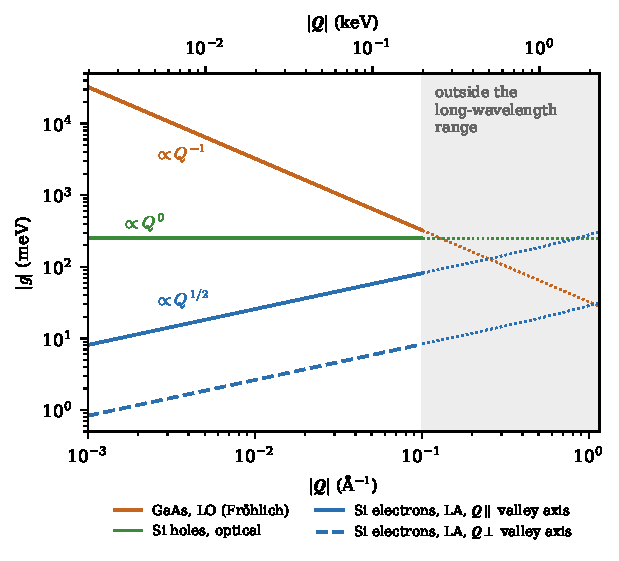
\includegraphics[width=0.72\linewidth]{figures/ch06/fig6_2.pdf}
  \caption{Magnitude of the electron--phonon vertex $|g|$, in the normalization in which $H_{\mathrm{ep}}$ carries $N^{-1/2}$, against the phonon wavevector $|\vect{Q}|$ (bottom axis in \si{\angstrom^{-1}}, top axis in keV), for the three long-wavelength forms of this section. Orange: Fr\"ohlich vertex \cref{eq:6.2-frohlich} of GaAs for an electron at the conduction-band minimum, with $\rho_{nn} = 1$ and the measured $\omega_{\mathrm{L}} = \SI{36.35}{meV}$, $\varepsilon_\infty = 10.88$, $\varepsilon_0 = 12.9$. Green: optical deformation potential \cref{eq:6.2-d} for the holes at the valence maximum of silicon, with the DFPT value \SI{10.45}{eV.\angstrom^{-1}} combined over the degenerate bands~\cite{li2021deformation} and $\omega = \SI{64.1}{meV}$. Blue: acoustic deformation potential \cref{eq:6.2-D} for an electron in a conduction valley of silicon and the longitudinal acoustic phonon, with $\vect{Q}$ along the valley axis (solid, $\Xi_d + \Xi_u = \SI{9.85}{eV}$) and perpendicular to it (dashed, $\Xi_d = \SI{1.01}{eV}$). These use the DFPT constants of Ref.~\cite{li2021deformation} and the DFPT longitudinal acoustic branch along $\mathrm{\Gamma}$--X of \cref{fig:5-si}, whose small-$Q$ slope is \SI{8.34}{km.s^{-1}} (measured: \SI{8.43}{km.s^{-1}}). The curves are these limiting forms, not vertices computed point by point. They are drawn solid up to \SI{0.1}{\angstrom^{-1}}, the end of the range over which the acoustic vertices of silicon were computed and found linear in $Q$~\cite[Fig.~5]{li2021deformation}. Beyond it they are dotted, in the shaded region up to the zone boundary of silicon at $2\pi/a = \SI{1.157}{\angstrom^{-1}}$. On logarithmic axes the slopes $-1$, 0 and $\tfrac12$ distinguish the polar, optical and acoustic couplings.}
  \label{fig:6-gQ}
\end{figure}

\subsection{Wannier interpolation of the vertex}

A phonon-assisted rate in silicon with an energy resolution of \SI{14}{meV} needs the vertex at about $4\times10^9$ pairs $(\vect{k},\vect{Q})$, for every pair of bands and every branch (\cref{app:E.5}). Density-functional perturbation theory costs about one ground-state calculation per phonon wavevector, and a few hundred wavevectors, a $6^3$ or $8^3$ grid, are what a calculation can afford. The step from such a \emph{coarse grid} to the \emph{fine grids} of a rate is an interpolation, and it works for the same reason as the interpolation of bands in \cref{sec:3.6}: in a suitable real-space representation the vertex is short-ranged.

The representation uses Wannier functions for the electrons and single displaced atoms for the phonons. We insert the Bloch sums of Wannier functions of one gauge, $\psi_{n\vect{k}} = N^{-1/2}\sum_{\vect{R}}\ee^{\ii\vect{k}\cdot\vect{R}}\sum_{n'}w_{n'}(\vect{r} - \vect{R})\,U^\dagger_{n'n}(\vect{k})$ (\cref{eq:A.5-wannier} inverted), into the matrix element of $\partial_{\kappa\alpha,\vect{Q}}V_{\mathrm{KS}} = \sum_{\vect{R}_p}\ee^{\ii\vect{Q}\cdot\vect{R}_p}\,\partial V_{\mathrm{KS}}/\partial u^\alpha_{\vect{R}_p\kappa}$. We then translate every term by the cell of the bra and sum over that cell, which cancels the factor $1/N$. What is left is
\begin{gather}
  \bigl\langle\psi_{m,\vect{k}+\vect{Q}}\bigr|\partial_{\kappa\alpha,\vect{Q}}V_{\mathrm{KS}}\bigl|\psi_{n\vect{k}}\bigr\rangle
  = \sum_{\vect{R}_e\vect{R}_p}\ee^{\ii(\vect{k}\cdot\vect{R}_e + \vect{Q}\cdot\vect{R}_p)}\,
  \bigl[U(\vect{k}+\vect{Q})\,g^W_{\kappa\alpha}(\vect{R}_e,\vect{R}_p)\,U^\dagger(\vect{k})\bigr]_{mn} ,
  \nonumber\\
  g^W_{m'n'\kappa\alpha}(\vect{R}_e,\vect{R}_p) = \Bigl\langle w_{m'}(\vect{r})\Bigr|\frac{\partial V_{\mathrm{KS}}}{\partial u^\alpha_{\vect{R}_p\kappa}}\Bigl|w_{n'}(\vect{r} - \vect{R}_e)\Bigr\rangle .
  \label{eq:6.2-gW}
\end{gather}
The real-space vertex $g^W$ is the matrix element, between a Wannier function at the origin and one in cell $\vect{R}_e$, of the screened potential change when a single atom in cell $\vect{R}_p$ moves. Multiplying by the polarization factors of \cref{eq:A.6-g} gives \cref{eq:E.5-ginterp}, and on the coarse grids the relation is inverted by a discrete Fourier transform, as for $H^W(\vect{R})$ in \cref{eq:3.6-HWR}. This is the scheme of Giustino, Cohen and Louie~\cite{giustino2007electron}, reviewed in Ref.~\cite[Eqs.~(177)--(179)]{giustino2017electron} and implemented in the Electron--Phonon Wannier (EPW) code~\cite{ponce2016epw}.

The real-space vertex decays in both of its lattice vectors. In $\vect{R}_e$ it decays as the overlap of two Wannier functions does, exponentially for the smooth gauges of \cref{sec:3.6}, because both must reach the region where the potential changes. In $\vect{R}_p$ it decays as the screened potential of one displaced atom, seen from the Wannier function at the origin. In a nonpolar insulator this potential has neither a monopole, since the displaced atom is screened to neutrality, nor a dipole, since $Z^* = 0$. It still has a quadrupole, and the vertex falls off as $R_p^{-3}$, a tail of no finite range whose Fourier transform carries a term of order $Q^0$ that depends on the direction of $\vect{Q}$. In silicon this quadrupolar part is small, and it can be subtracted like the dipole of a polar crystal below. By the argument that led to \cref{eq:3.6-exact}, a coarse grid whose supercell contains the short-ranged remainder of $g^W$ reproduces the vertex everywhere, and the tails beyond it set the error. For diamond and silicon a $6^3$ or $8^3$ coarse grid of phonon wavevectors is enough (\cref{app:E.5}).

A polar crystal breaks the argument. The displaced atom carries the dipole $eZ^*_\kappa\cdot\vect{u}$ screened by $\varepsilon_\infty$, its potential falls off as $R_p^{-2}$, and the Fourier transform of that tail is the $1/Q$ singularity of the Fr\"ohlich vertex. No finite sum of Fourier components reproduces a singularity. The remedy is the one that \cref{sec:5.5} used for the nonanalytic part of the dynamical matrix. The long-range vertex is known in closed form from $Z^*_\kappa$ and $\varepsilon_\infty$ alone, \cref{eq:D.14-gL} or its version with the sum over reciprocal-lattice vectors, \cref{eq:E.5-gL}. One subtracts it from the coarse-grid vertices, interpolates the short-range remainder $g^{\mathrm{S}} = g - g^{\mathrm{L}}$, which is as smooth as the vertex of a nonpolar crystal, and adds $g^{\mathrm{L}}$ back analytically at every fine-grid point~\cite{verdi2015frohlich}. The split $g = g^{\mathrm{S}} + g^{\mathrm{L}}$ is not unique, since any smooth function can be moved from one part to the other, but every choice puts the whole singularity into $g^{\mathrm{L}}$, and that is all the interpolation needs. The density vertex in $g^{\mathrm{L}}$ is needed at the fine-grid points too, and at small $\vect{Q}$ it is $[U(\vect{k}+\vect{Q})U^\dagger(\vect{k})]_{mn}$ in the Wannier gauge, so that $g^{\mathrm{S}}$ and $g^{\mathrm{L}}$ carry the same phases (\cref{app:A.5}). The quadrupolar terms, present in silicon as in GaAs and, together with the Born charges, the origin of the piezoelectric vertex of GaAs, are long-ranged in the same way and are subtracted with the dipole where the code allows it (\cref{app:E.5}).

\begin{figure}[tbp]
  \centering
  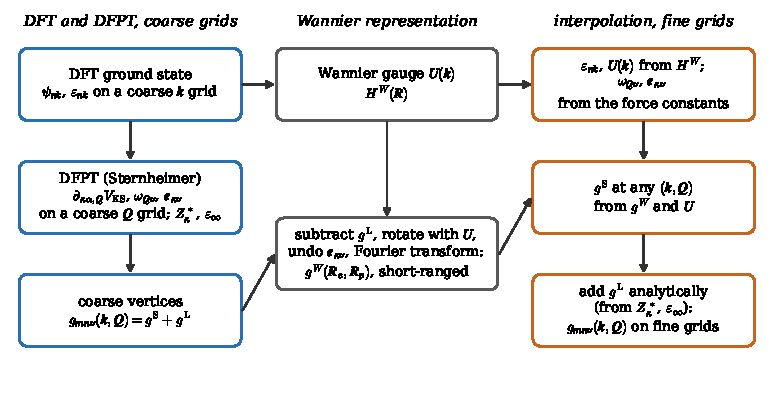
\includegraphics[width=\linewidth]{figures/ch06/fig6_3.pdf}
  \caption{From first principles to interpolated electron--phonon vertices. Left: a density-functional calculation on a coarse grid of crystal momenta gives the Bloch states and energies. Density-functional perturbation theory on a coarse grid of phonon wavevectors gives the screened potential changes $\partial_{\kappa\alpha,\vect{Q}}V_{\mathrm{KS}}$, the phonons, and in a polar crystal $Z^*_\kappa$ and $\varepsilon_\infty$. Their matrix elements are the coarse vertices, \cref{eq:6.2-g}. Middle: the Bloch states define the Wannier gauge $U(\vect{k})$; the long-range part $g^{\mathrm{L}}$ is subtracted, and the rotated remainder is transformed to the real-space vertex $g^W(\vect{R}_e,\vect{R}_p)$ of \cref{eq:6.2-gW}, short-ranged in both lattice vectors. Right: the real-space Hamiltonian and force constants give bands, gauge matrices and phonons at any point; $g^W$ is transformed back, \cref{eq:E.5-ginterp}, and $g^{\mathrm{L}}$, \cref{eq:E.5-gL}, is added analytically. Every quantity in one amplitude uses the same $U(\vect{k})$.}
  \label{fig:6-chain}
\end{figure}

\Cref{fig:6-chain} summarizes the chain. Its pitfalls are practical: a Wannier manifold that misses the states a rate needs, a coarse grid that misplaces the conduction minimum of silicon, a gauge that differs between $g$ and $\rho$. \Cref{app:E.5} discusses each, with the grid sizes, the counts of matrix elements and the checks against direct DFPT at points off the coarse grid. The result is a vertex at any $(\vect{k},\vect{Q})$ for about the cost of a few hundred phonon calculations.
